\documentclass{article}[12pt]
\usepackage{color,amsmath,amssymb,graphicx,fancyhdr,amsfonts,amsthm,algorithmic,verbatim,bbold,environ}
\usepackage{algorithm,hyperref}
\usepackage{mkolar_definitions}
\usepackage{multirow}
\usepackage{diagbox}
\usepackage{longtable,booktabs}
\usepackage{geometry}
\usepackage{subfigure} 
\numberwithin{algorithm}{section}

\newcommand{\tightlist}{%
  \setlength{\itemsep}{0pt}\setlength{\parskip}{0pt}}


\geometry{a4paper,scale=0.8}


\title{PI-Measure: A Set-Theoretic View of Partial Information}

\author{Litao Zhou, Hongbo Yang, Shiwen Dong}
\date{\today}

\usepackage[hyperref=true,backend=biber,sorting=none,backref=true]{biblatex}
\addbibresource{ref.bib}

\begin{document}

\maketitle

\section{Introduction}

% 研究意义,前人工作
% 研究方法,主要创新点
% 论文组织结构


\qquad Developing from investigation in physics, engineering and mathematics, information theory originated from Shannon's pioneering research of the reliability and coding in communication system. It has successfully become a universal tool for analyzing complex systems, and has been applied in many fields such as genetics, physics, neuroscience, machine learning and so on. Shannon’s mutual information is by far the most widely used concept from the information theory \cite{shannon1948mathematical}, and Shannon’s information measures refer to entropy, conditional entropy, mutual information, and conditional mutual information, which are the most significant measures of information in information theory. 


The relations between the entropies, conditional entropies and mutual information for two random variables X and Y can be summarized by a variation of the Venn diagram. With the help of such diagram, the relations can be depicted intuitively and vividly, thus reducing the difficulty of readers' understanding of the knowledge. This one-to-one correspondence between Shannon’s information measures and set theory is not just a coincidence for two random variables. Actually, Shannon’s information measures for any n $\geq$ 2 random variables all have a set-theoretic structure.

Using a few basic concepts in measure theory such as fields, atoms and signed measure $\mu$, a theory “I-measure” which establishes a one-to-one correspondence between Shannon’s information measures and set theory in full generality has been developed \cite{yeung2008information,yeung2012first}. Then manipulations of Shannon’s information measures can be viewed as set operations, thus allowing the rich suite of tools in set theory to be used in information theory. Moreover, the structure of Shannon’s information measures can easily be visualized by means of an information diagram if four or fewer random variables are involved. The use of information diagrams simplifies many difficult proofs in information theory problems. More importantly, these results, which may be difficult to discover in the first place, can easily be obtained by inspection of an information diagram.

Until now, most of the work of information theory only deals with the simplest case: the information about another variable provided by one variable. By contrast, most challenging scientific problems, such as many-body problems in physics \cite{belyaev1959many}, and population coding in neuroscience \cite{Dayan2001Theoretical,Rieke1996Spikes}, involve understanding the structure of interactions between three or more variables. To generalize information theory to multivariate interactions, interaction information was proposed as a measure of the amount of information bound in a set of variables, rather than the amount of information existing in any subset of those variables.  So entropy and mutual information correspond to the first- and second-order interaction information, while interaction information and its third-order, fourth-order and higher-order variants provide a method to represent the structure of multivariate information. However, the widespread use of interactive information is largely hindered by "odd" and "unfortunate" attributes. For three or more variables, interaction information can be negative, whose meaning is usually unclear for information as it is commonly understood.

Then a new perspective on the structure of multivariate information has been formulated.\cite{Williams2010Nonnegative} Considering the general structure of the information that a set of sources provide about a given variable, a new definition of redundancy was proposed, which can be used to exhaustively decompose the Shannon information in a multivariate system into partial information atoms.

Here we use the above-mentioned method of I-measure, aiming to establish a one-to-one correspondence between partial information measures and the set theory. With this correspondence, manipulations of partial information measures can be viewed as set operations. What’s more, the structure of partial information measures can be easily visualized by a partial information diagram. And we hope that this can simplify the deduction and  proofs in information theory problems.



\section{I-Measure}
We have already known that the Venn diagrams can give us a clear picture of the relations among sets. In order to construct  similar information diagrams to facilitate our analysis of information, we need to introduce a method to connect Shannon's information measure with things in set theory. We introduce a few basic concepts in measure theory which will be used subsequently. These concepts will be illustrated by simple examples.\\

\begin{definition}[Field]\label{field}
The field $\mathcal{F}_{n}$ generated by sets $\tilde{X}_{1}, \tilde{X}_{2}, \cdots, \tilde{X}_{n}$ is the collection of sets which can be obtained by any sequence of usual set operations (union, intersection, complement, and difference) on $\tilde{X}_{1}, \tilde{X}_{2}, \cdots, \tilde{X}_{n}$\\
\end{definition}

\begin{definition}[Atom]\label{atom}
The atoms of $\mathcal{F}_{n}$ are sets of the form $\cap_{i=1}^{n} Y_{i},$ where $Y_{i}$ is either$\tilde{X}_{i}$ or $\tilde{X}_{i}^{c},$ the complement of $\tilde{X}_{i}$\\
\end{definition}

\begin{definition}[Signed Measure]\label{sm}
A real function $\mu$ defined on $\mathcal{F}_{n}$ is called a signed measure if it is set-additive, i.e., for disjoint $A$ and $B$ in $\mathcal{F}_{n}$
\begin{equation}
\mu(A \cup B)=\mu(A)+\mu(B)
\end{equation}
\end{definition}

For a signed measure $\mu,$ we have
\begin{equation}
\mu(\emptyset)=0
\end{equation}
which can be seen as follows. For any $A$ in $\mathcal{F}_{n}$
\begin{equation}
\mu(A)=\mu(A \cup \emptyset)=\mu(A)+\mu(\emptyset)
\end{equation}
by set-additivity because $A$ and $\emptyset$ are disjoint. A signed measure $\mu$ on $\mathcal{F}_{n}$ is completely specified by its values on the atoms of $\mathcal{F}_{n} .$ The values of $\mu$ on the other sets in $\mathcal{F}_{n}$ can be obtained via set-additivity.

Until now, we have found a practical method to measure a set. We'll see how we can introduce a measure for the information in section \ref{sec2.1}.


\begin{figure}[ht]
 
\centering
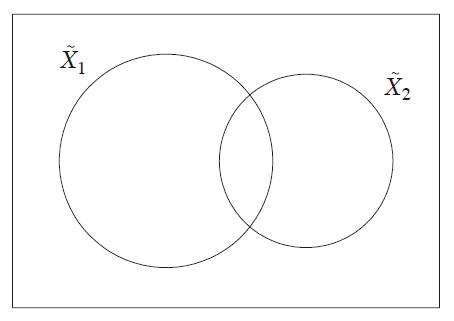
\includegraphics[scale=0.4]{tex/Im1.png}
\caption{The Venn diagram for $\tilde{X}_{1}$ and $\tilde{X}_{2}$}
\label{im1}
 
\end{figure}

\subsection{I-Measure between 2 R.V.s}
\label{sec2.1}

To start with, we first formulate the one-to-one correspondence
between Shannon's information measures and set theory for two random variables. For random variables ${X}_1$ and ${X}_2$, let $\tilde{X}_{1}$ and $\tilde{X}_{2}$ be sets respectively corresponding to ${X}_1$ and ${X}_2$. The sets $\tilde{X}_{1}$ and $\tilde{X}_{2}$ generates the field $\mathcal{F}_{n}$ whose
atoms are 

$$\tilde{X}_{1} \cap \tilde{X}_{2}, \tilde{X}_{1}^{c} \cap \tilde{X}_{2}, \tilde{X}_{1} \cap \tilde{X}_{2}^{c}, \tilde{X}_{1}^{c} \cap \tilde{X}_{2}^{c}$$
Their relationship is shown by a Venn diagram in Figure \ref{im1}.

  In our formulation, we set the universal set $\Omega$ to $\tilde{X}_{1} \cup \tilde{X}_{2}$. With this choice of $\Omega,$ the Venn diagram for $\tilde{X}_{1}$ and $\tilde{X}_{2}$ is represented by the diagram in Figure \ref{im2}. For simplicity, the sets $\tilde{X}_{1}$ and $\tilde{X}_{2}$ are respectively labeled by $X_{1}$ and $X_{2}$ in the diagram. We call this the information diagram for the random variables $X_{1}$ and $X_{2} .$ In this diagram, the universal set, which is the union of $\tilde{X}_{1}$ and $\tilde{X}_{2}$ is not shown explicitly just as in a usual Venn diagram. Note that with our choice of the universal set, the atom $\tilde{X}_{1}^{c} \cap \tilde{X}_{2}^{c}$ degenerates to the empty set.
  
\begin{figure}[ht]
 
\centering
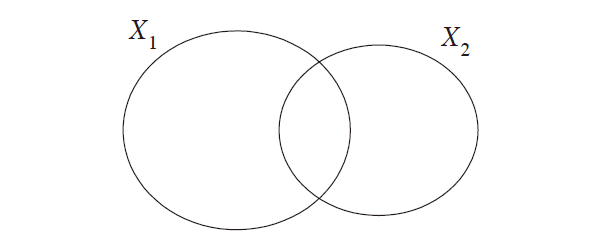
\includegraphics[scale=0.4]{tex/Im2.png}
\caption{The information diagram for ${X}_{1}$ and
${X}_{2}$}
\label{im2}
 
\end{figure}

From what we know about random variables $X_{1}$ and $X_{2}$, we can explicit the Shannon's information measures
\[
H\left(X_{1}\right), H\left(X_{2}\right), H\left(X_{1} | X_{2}\right), H\left(X_{2} | X_{1}\right), H\left(X_{1}, X_{2}\right), I\left(X_{1} ; X_{2}\right)
\]
Writing $A \cap B^{c}$ as $A-B,$ we now define a signed measure $\mu^{*}$ by
\begin{equation}
    \mu^{*}\left(\tilde{X}_{1}-\tilde{X}_{2}\right)=H\left(X_{1} | X_{2}\right)
\end{equation}
\begin{equation}
\mu^{*}\left(\tilde{X}_{2}-\tilde{X}_{1}\right)=H\left(X_{2} | X_{1}\right)
\end{equation}
and
\begin{equation}
\mu^{*}\left(\tilde{X}_{1} \cap \tilde{X}_{2}\right)=I\left(X_{1} ; X_{2}\right)
\end{equation}
These are the values of $\mu^{*}$ on the nonempty atoms of $\mathcal{F}_{2}$ (i.e., atoms of $\mathcal{F}_{2}$ other $\left.\operatorname{than} \tilde{X}_{1}^{c} \cap \tilde{X}_{2}^{c}\right) .$ The values of $\mu^{*}$ on the other sets on $\mathcal{F}_{2}$ can be obtained via set-additivity. In particular, we can easily formulate these following relations
\begin{equation}
\mu^{*}\left(\tilde{X}_{1} \cup \tilde{X}_{2}\right) =H\left(X_{1}, X_{2}\right)
\end{equation}

\begin{equation}
\mu^{*}\left(\tilde{X}_{1}\right) =H\left(X_{1}\right)
\end{equation}

and
\begin{equation}
\mu^{*}\left(\tilde{X}_{2}\right)=H\left(X_{2}\right)
\end{equation}



For example, $\mu^{*}\left(\tilde{X}_{1} \cup \tilde{X}_{2}\right)$ can be calculated by
\begin{align}
&\mu^{*}\left(\tilde{X}_{1} \cup \tilde{X}_{2}\right)\\
&=\mu^{*}\left(\tilde{X}_{1}-\tilde{X}_{2}\right)+\mu^{*}\left(\tilde{X}_{2}-\tilde{X}_{1}\right)+\mu^{*}\left(\tilde{X}_{1} \cap \tilde{X}_{2}\right)\\
&=H\left(X_{1} | X_{2}\right)+H\left(X_{2} | X_{1}\right)+I\left(X_{1} ; X_{2}\right) \\
&=H\left(X_{1}, X_{2}\right) 
\end{align}


By now, the relationship between Shannon's information measures and signed measure (i.e. the set theory) is clear for 2 R.V.s. By the approach of sign mapping, we can change between Shannon's information measures into signed measure, and vice versa. 



 \subsection{\protect\boldmath Construction of  \texorpdfstring{$\mu^{*}$}{\textmu*}}
 
 In this section, we are finding a more general conclusion, which means to find a similar relation in a higher random variable space. For n $\geq$ 2, consider n random variables ${X}_{1}$;${X}_{2}$; ... ;${X}_{n}$. For any random variable X,
let $\tilde{X}$ be a set corresponding to X. Let
\begin{equation}
    \mathcal{N}_{n}=\{1,2, \cdots, n\}
\end{equation}
Define the universal set $\Omega$ to be the union of the sets$\tilde{X}_{1}, \tilde{X}_{2}, \cdots, \tilde{X}_{n},$ i.e.
\begin{equation}
    \Omega=\bigcup_{i \in \mathcal{N}_{n}} \tilde{X}_{i}
\end{equation}
And we use $\mathcal{F}_{n}$ to denote the field generated by $\tilde{X}_{1}, \tilde{X}_{2}, \cdots, \tilde{X}_{n} .$\\

The set
\[
A_{0}=\bigcap_{i \in \mathcal{N}_{n}} \tilde{X}_{i}^{c}
\]   
is called the empty atom of $\mathcal{F}_{n}$ because

\begin{equation}
    \bigcap_{i \in \mathcal{N}_{n}} \tilde{X}_{i}^{c}=\left(\bigcup_{i \in \mathcal{N}_{n}} \tilde{X}_{i}\right)^{c}=\Omega^{c}=\emptyset
\end{equation}


All the atoms of $\mathcal{F}_{n}$ other than $A_{0}$ are called nonempty atoms.\\
 
 To simplify notation, we will use $X_{G}$ to denote $\left(X_{i}, i \in G\right)$ and $\tilde{X}_{G}$ to denote $\cup_{i \in G} \tilde{X}_{i}$ for any nonempty subset $G$ of $\mathcal{N}_{n}$\\
 

\begin{theorem}\label{th1}
Let
\begin{equation}
    \mathcal{B}=\left\{\tilde{X}_{G}: G \text { is a nonempty subset of } \mathcal{N}_{n}\right\}
\end{equation}
Then a signed measure $\mu$ on $\mathcal{F}_{n}$ is completely specified by $\{\mu(B), B \in \mathcal{B}\}$
which can be any set of real numbers.
\end{theorem}
When introducing our work of "PI-Measure", we will use a similar way as this proof to show a connection in $\mu^{*}$ and decomposed mutual information, and that proof will be given.


Until now the work to expand signed measures into higher space is finished. Next we'll look at how to substitute signed measures into Shannon's information measure when n $\geq$ 2.\\

We now construct the I-Measure $\mu^{*}$ on $\mathcal{F}_{n}$ using Theorem \ref{th1} by defining%%%%%%%%%%%%%
\begin{equation}
    \mu^{*}\left(\tilde{X}_{G}\right)=H\left(X_{G}\right)
\end{equation}
for all nonempty subsets $G$ of $\mathcal{N}_{n} .$ In order for $\mu^{*}$ to be meaningful, it has to be consistent with all Shannon's information measures. In that case, the following must hold for all (not necessarily disjoint $)$ subsets $G, G^{\prime}, G^{\prime \prime}$ of $\mathcal{N}_{n}$ where $G$ and $G^{\prime}$ are nonempty:
\begin{equation}\label{eqx1}
    \mu^{*}\left(\tilde{X}_{G} \cap \tilde{X}_{G^{\prime}}-\tilde{X}_{G^{\prime \prime}}\right)=I\left(X_{G} ; X_{G^{\prime}} | X_{G^{\prime \prime}}\right)
\end{equation}
When $G^{\prime \prime}=\emptyset,(\ref{eqx1})$ becomes
\begin{equation}
\mu^{*}\left(\tilde{X}_{G} \cap \tilde{X}_{G^{\prime}}\right)=I\left(X_{G} ; X_{G^{\prime}}\right)
\end{equation}
When $G=G^{\prime},(\ref{eqx1})$ becomes
\begin{equation}
\mu^{*}\left(\tilde{X}_{G}-\tilde{X}_{G^{\prime \prime}}\right)=H\left(X_{G} | X_{G^{\prime \prime}}\right)
\end{equation}
When $G=G^{\prime}$ and $G^{\prime \prime}=\emptyset,(\ref{eqx1})$ becomes
\begin{equation}
    \mu^{*}\left(\tilde{X}_{G}\right)=H\left(X_{G}\right)
\end{equation}

From these cases we know that (\ref{eqx1}) can cover all the 4 conditions that Shannon's information measure may have. Thus, we can say that Equation (\ref{eqx1}) holds, if and only if $\mu^{*}$ is consistent with all Shannon's information measures.

\begin{theorem} $\mu^{*}$ is the unique signed measure on $\mathcal{F}_{n}$ which is consistent with all Shannon's information measures.
\end{theorem}

Proof. Consider
\[
\begin{array}{l}
\mu^{*}\left(\tilde{X}_{G} \cap \tilde{X}_{G^{\prime}}-\tilde{X}_{G^{\prime \prime}}\right) \\
=\mu^{*}\left(\tilde{X}_{G \cup G^{\prime \prime}}\right)+\mu^{*}\left(\tilde{X}_{G^{\prime} \cup G^{\prime \prime}}\right)-\mu^{*}\left(\tilde{X}_{G \cup G^{\prime} \cup G^{\prime \prime}}\right)-\mu^{*}\left(\tilde{X}_{G^{\prime \prime}}\right) \\
=H\left(X_{G \cup G^{\prime \prime}}\right)+H\left(X_{G^{\prime} \cup G^{\prime \prime}}\right)-H\left(X_{G \cup G^{\prime} \cup G^{\prime \prime}}\right)-H\left(X_{G^{\prime \prime}}\right) \\
=I\left(X_{G} ; X_{G^{\prime}} | X_{G^{\prime \prime}}\right)
\end{array}
\]
i.e., $\mu^{*}$ is consistent with all Shannon's information measures. In order that $\mu^{*}$ is consistent with all Shannon's information measures, for all nonempty subsets $G$ of $\mathcal{N}_{n}, \mu^{*}$ has to satisfy Equation (\ref{eqx1}), which in fact is the definition of $\mu^{*}$. Therefore, $\mu^{*}$ is the unique signed measure on $\mathcal{F}_{n}$ which is consistent with all Shannon's information measures.

 \subsection{Markov Chain, a Special Case}
\label{sec:markov}
 
 
 
All the contents above together, give us the possibility to draw a clear picture of the relationship among Shannon's information measure of discrete random variables. (The n = 3 case is shown below)
\begin{figure}[ht]
 
\centering
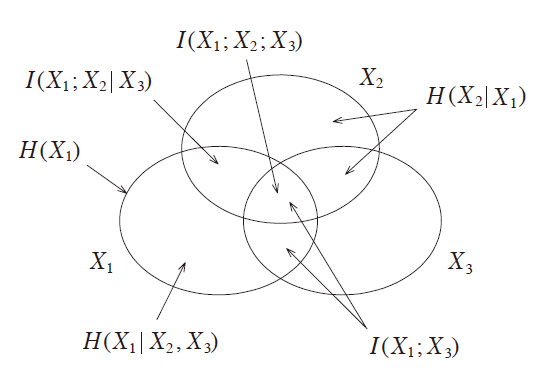
\includegraphics[scale=0.4]{tex/Im3.png}
\caption{The information diagram for ${X}_{1}$, ${X}_{2}$ and ${X}_{3}$}
\label{im3}
 
\end{figure}


In this section, we'll focus on a special case of this relation, i.e. the Markov Chain (MC). We explore the structure of Shannon's information measures when $X_{1} \rightarrow X_{2} \rightarrow \cdots \rightarrow X_{n}$ forms a Markov chain. To start with, we consider $n=3,$ i.e., $X_{1} \rightarrow X_{2} \rightarrow X_{3}$ forms a Markov chain. since
\[
\mu^{*}\left(\tilde{X}_{1} \cap \tilde{X}_{2}^{c} \cap \tilde{X}_{3}\right)=I\left(X_{1} ; X_{3} | X_{2}\right)=0
\]
the atom $\tilde{X}_{1} \cap \tilde{X}_{2}^{c} \cap \tilde{X}_{3}$ does not have to be displayed in an information diagram. Therefore, in constructing the information diagram, the regions representing the random variables $X_{1}, X_{2},$ and $X_{3}$ should overlap with each other such that the region corresponding to the atom $\tilde{X}_{1} \cap \tilde{X}_{2}^{c} \cap \tilde{X}_{3}$ is empty, while the regions corresponding to all other nonempty atoms are nonempty. Figure 3.7 shows such a construction, in which each random variable is represented by a "mountain." From Figure 3.7, we see that $\tilde{X}_{1} \cap \tilde{X}_{2} \cap \tilde{X}_{3},$ as the only atom on which $\mu^{*}$ may take a negative value, now becomes identical to the atom $\tilde{X}_{1} \cap \tilde{X}_{3} .$ Therefore, we have
\[
\begin{aligned}
I\left(X_{1} ; X_{2} ; X_{3}\right) &=\mu^{*}\left(\tilde{X}_{1} \cap \tilde{X}_{2} \cap \tilde{X}_{3}\right) \\
&=\mu^{*}\left(\tilde{X}_{1} \cap \tilde{X}_{3}\right) \\
&=I\left(X_{1} ; X_{3}\right) \\
& \geq 0
\end{aligned}
\]
%%%%%%%%%%%%%%%%%%%
%%%%%%%%%%%%%%%%%%%%%%%%%%%%%%%%%%%%%%
%%%%%%%%%%%%%%%%%%%%%%%%%%%%%%%%%%%%%%
%%%%%%%%%%%%%%%%%%%%%%%%%%%%%%%%%%%%%%
%%%%%%%%%%%%%%%%%%%%%%%%%%%%%%%%%%%%%%




 Information Diagrams for Zero Measure
In Markov Chain $X_{1} \rightarrow X_{2} \rightarrow X_{3}$, since \begin{equation}\mu^{*}\left(\tilde{X}_{1} \cap \tilde{X}_{2}^{c} \cap \tilde{X}_{3}\right)=I\left(X_{1} ; X_{3} | X_{2}\right)=0\end{equation}
        We don't have to plot that region out in the information diagram, making the diagram simpler and more useful when reasoning about Shannon information measures. And for MC with 4 or more R.V.s, we can also find out that some parts needn't to be plotted, because of the properties of Markov Chain.


Above all, we've introduced several general ideas in constructing the correspondence between set theory and Shannon information. These ideas will be revisited later , helping us find a correspondence between another type of information measure and set theory.



\section{Decomposition of Multivariate Information}
\subsection{The Structure of Multivariate Information}
Suppose there is a random variable $S$ whose information is provided by a random  $\mathbf{R}=\left({R}_1,{R}_2,\ldots,{R}_{n-1}\right)$, then we try to decompose the information into some information contributed by the subsets of $\mathbf{R}$ individually or jointly.

Consider the case where $\mathbf{R}=\left({R}_1,{R}_2\right)$. The total information ${R_1}$ and ${R_2}$ provided is the mutual
information  $I\left(S;{R}_1,{R}_2\right)$, and their contributions can be divided into three parts. First, the unique information, which means the information only provided by ${R_1}$, or vice versa. Second, the redundancy, which means the same or overlapping information that ${R_1}$ and ${R_2}$ provide. Third, the synergy, which means the information that is provided by the combination of ${R_1}$ and ${R_2}$ while not available from either alone.

Therefore, as is shown in Figure \ref{figl}, the total information can be decomposed into three parts: the synergistic information contributed jointly by ${R_1}$ and ${R_2}$,  the unique information from ${R_1}$ or ${R_2}$, and the redundant information shared by ${R_1}$ and ${R_2}$. So we can identify them as the basic atoms of multivariate information.


 
\begin{figure}[ht]
 
\centering
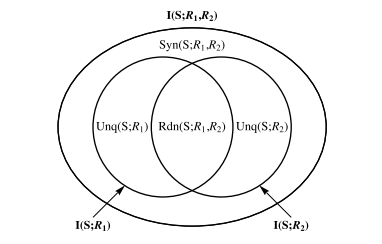
\includegraphics[scale=0.6]{tex/structure3.png}
\caption{Structure of multivariate information for 3 variables}
\label{figl}
 
\end{figure}



Actually, the unique information can be considered as a deformation of synergy or redundancy, so we can say that the multivariate information constitutes of redundancy and synergy.



% 引入我们讨论的信息量
% 给出关键性质


\subsection{Redundancy Measure}

To formally measure the redundancy between multiple collections of sources, we now introduce a redundancy measure $I_{\min}$. Let $A_1, A_2, \ldots, A_k$ be nonempty and potentially overlapping subsets of $\mathbf{R},$ which we call sources. We introduce $I_{\min}$ to measure the information that all sources provide about $S$.

While the specific information $I(S=s ; \mathbf{A})$ quantifies the information associated with a particular outcome of $S$, $I_{\min}$ describes all sources offer to S, or we say "redundancy". Various definitions of specific information have been proposed to quantify different relationships between $S$ and $\mathbf{A}$ but for our purposes the most useful is
\begin{equation}
I(S=s ; \mathbf{A})=\sum_{\mathbf{a}} p(\mathbf{a} | s)\left[\log\frac{1}{p(s)}-\log\frac{1}{p(s |\mathbf{a})}\right]
\end{equation}

To better introduce the meaning of this definition, we use $\frac{1}{p(s)}$ instead of ${p(s)}$. And the former one is called the surprise of $s,$ so $I(S=s ; \mathbf{A})$ is the average reduction in surprise of $s$ given knowledge of $\mathbf{A} .$ In other words, $I(S=s ;\mathbf{ A}$ quantifies the information that $\mathbf{A}$ provides about each particular outcome $s \in S,$ while $I(S ; \mathbf{A})$ is the expected value of this quantity over all outcomes of $S$. Given these considerations, a natural measure of redundancy is the expected value of the minimum information that any source provides about each outcome of $S$.
\begin{definition}[Redundancy Measure]
\begin{equation}I_{\min }\left(S ;\left\{\mathbf{A}_{1}, \mathbf{A}_{2}, \ldots, \mathbf{A}_{k}\right\}\right)=\sum_{s} p(s) \min _{\mathbf{A}_{i}} I\left(S=s ; \mathbf{A}_{i}\right)\end{equation}
where the domain of $I_{\min}$ $\mathcal{A}(\mathbf{R})=\left\{\alpha \in \mathcal{P}_{1}\left(\mathcal{P}_{1}(\mathbf{R})\right): \forall \mathbf{A}_{i}, \mathbf{A}_{j} \in \alpha, \mathbf{A}_{i} \notin \mathbf{A}_{j}\right\}$
\end{definition}
$I_{\min }$ captures the idea that redundancy is the information common to all sources (the minimum information that any source provides $),$ while taking into account that sources may provide information about different outcomes of $S$. Note that, like the mutual information, $I_{\min }$ is also an expected value of specific information terms. And similarly to $I$, $I_{\min }$ also has several useful properties that can be easily proved from its definition.
\begin{itemize}
    \item $I_{\min}$ is non-negative
    \item $I_{\min }$ is less than or equal to $I\left(S ; \mathbf{A}_{i}\right)$ for all $\mathbf{A}_{i}$ 's
    \item For a given source A, the amount of information redundant with $\mathbf{A}$ is maximal for $I_{\min }(S ;\{\mathbf{A}\})=I(S ; \mathbf{A}) .$
\end{itemize}

These properties can confirm $I_{\min}$ with its interpretation as a measure of redundancy.





\subsection{Partial Information Decomposition}
\label{sec:partialdecompositon}

Note that $I_{\min}$ can measure redundancy between collections of sources like $\left\{\left\{R_{1}\right\},\left\{R_{2}, R_{3}\right\}\right\}$ denoted as $\{1\}\{23\}$. A natural observation is that, for any source sets in one collection, if its subsets can always be found at another collection, then it must measure a greater redundancy over the other collection. Therefore, we can define a partial order over the elements of $A(R)$ such that one is considered to precede another if and only if the latter provides any redundant information that the former provides. Formally,
    \begin{equation}\forall \alpha, \beta \in \mathcal{A}(\mathbf{R}), \alpha \preccurlyeq \beta \Leftrightarrow \forall \mathbf{B} \in \beta, \exists \mathbf{A} \in \alpha, \mathbf{A} \subseteq \mathbf{B}\label{partialorder}\end{equation}

And from this partial order, a lattice can be illustrated as follow, which gives us a clear picture of the partial order among collections of sources.(shown in Figure \ref{fig:lattice})



\begin{figure}
            \centering
            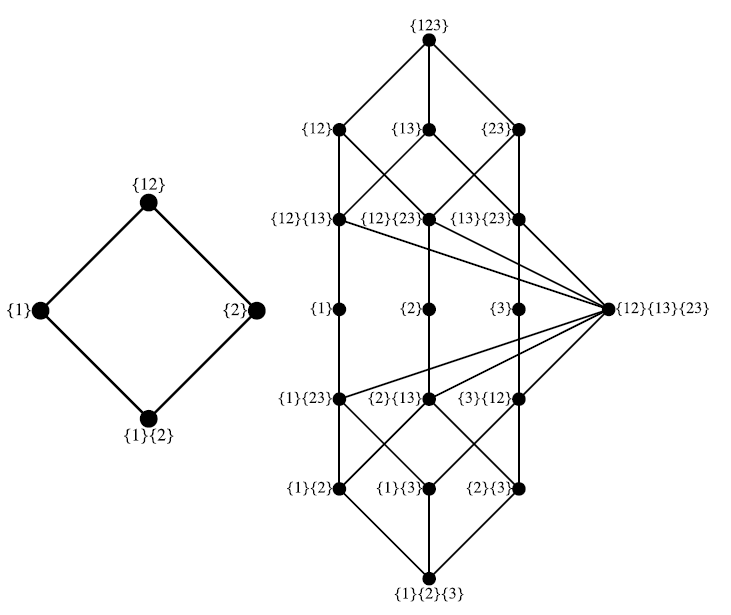
\includegraphics[width=0.6\linewidth]{img/lattic.png}
            \caption{Redundancy lattice for (A) 3 and (B) 4 variables.}
            \label{fig:lattice}
        \end{figure}

The redundant information associated with each node of the redundancy lattice includes, but is not limited to, the redundant information provided by all nodes lower in the lattice. Thus moving from node to node up the lattice, $I_{\min }$ can be thought of as a kind of "cumulative information function," effectively integrating the information provided by increasingly inclusive collections of sources.

The observation above implies that the nodes in the lattice actually would decompose redundancy measure into several non-intersecting fragments and derive an inverse of ${I}_{min}$ called the \textit{partial information function} (PI-function). Whereas ${I}_{min}$ quantifies cumulative information, the PI-function measures the partial information contributed uniquely by each particular collection of sources. This partial information will form the atoms into which we decompose the total information
that $\mathbf{R}$ provides about S. Formally, we define these components with the partial order defined in Equation  \ref{partialorder}.

\begin{definition}[Partial Information]For a collection of sources $\alpha \in \mathcal{A}(\mathbf{R}),$ the PI-function, denoted $\Pi_{\mathrm{R}},$ is defined implicitly by
\begin{equation}
    I_{\min }(S ; \alpha)=\sum_{\beta \preccurlyeq \alpha} \Pi_{\mathrm{R}}(S ; \beta)
    \label{def:partial}
\end{equation}


\end{definition}


The relationship between these measures can be shown in a partial information (PI) diagram, which is shown later. Formally, $\Pi_{\mathrm{R}}$ corresponds to the the Möbius inverse of $I_{\min }$ \cite{stanley1997enumerative}. And from this relationship, it is clear that $\Pi_{R}$ can be calculated recursively as
\begin{equation}
    \Pi_{\mathbf{R}}(S ; \alpha)=I_{\min }(S ; \alpha)-\sum_{\beta \prec \alpha} \Pi_{\mathbf{R}}(S ; \beta)
\end{equation}

Put into words, $\Pi_{\mathrm{R}}(S ; \alpha)$ quantifies the information provided redundantly by the sources of $\alpha$ that is not provided by any simpler collection of sources (i.e., any $\beta$ lower than $\alpha$ on the redundancy lattice shown above). \textbf{Note} that $\Pi_{\mathrm{R}}$ is non-negative, which proof can be seen in \cite{Williams2010Nonnegative}.

\label{thm:nonneg}

%%%%%%%%%%%%%%%%%%%%%



\begin{figure}
\centering
\subfigure[3 Variables]{
\begin{minipage}[t]{0.5\linewidth}
\centering
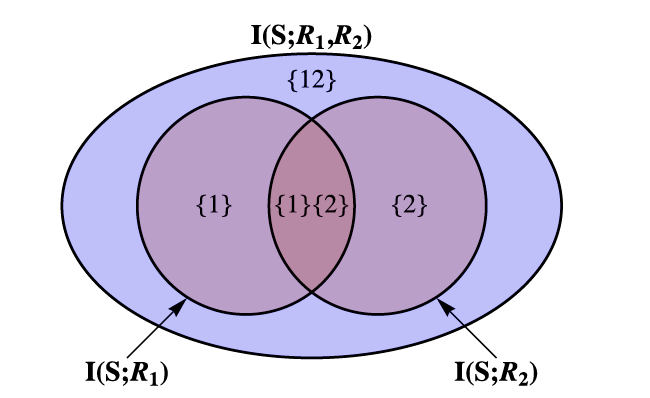
\includegraphics[height=5cm]{img/partial3.png}
%\caption{fig1}
\end{minipage}%
}%
\subfigure[4 Variables]{
\begin{minipage}[t]{0.5\linewidth}
\centering
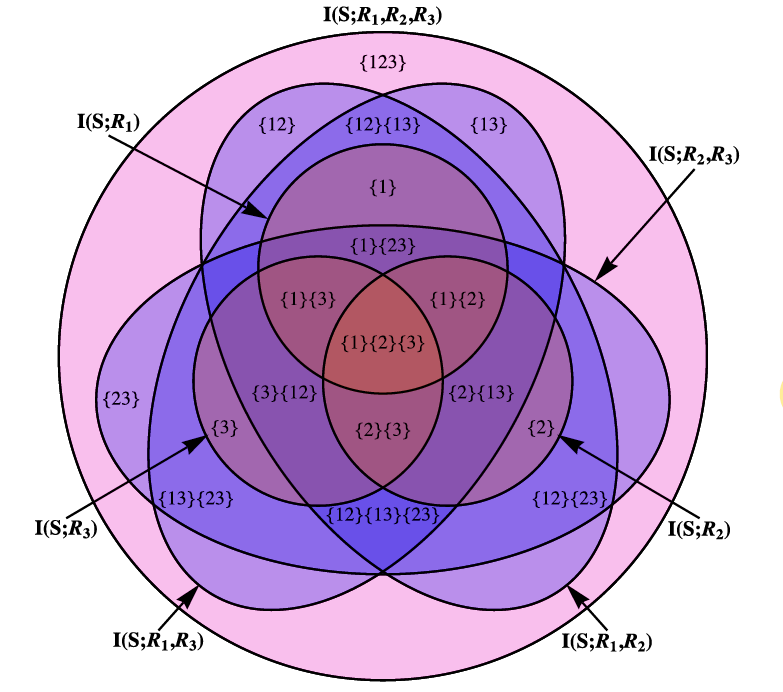
\includegraphics[height=5cm]{img/partial4.png}
%\caption{fig2}
\end{minipage}%
}%
\centering
\caption{Partial Information Diagrams}
\label{fig:pidiagram}
\end{figure}


Above all, we've formed a basic idea of the decomposition of partial information. We'll proceed to formulate how to measure these notions with set measure in the next chapter.






\section{PI-Measure}

We next show how redundancy measure can be formulated in a set-theoretic way. In this chapter, we develop a theory which establishes a one-to-one correspondence between set theory and partial information measures, as well as their decomposed values, namely $I_{\min}$ and $\Pi_{\mathbf{R}}$. Unlike the scenario where relationship between entropies and mutual information is formed, the correspondence here involves more atomic sets and more complicated set properties.

\subsection{Formulation}

In this section, using the notion of measure theory introduced in Chapter 2, % todo!!,
we will give a formal definition for the correspondence. To fix ideas, we first formulate in this section the one-to-one correspondence between redundancy measures and set theory for a three dimensional random source vector.

\paragraph{Field Generation}
For random variables $A_1$, $A_2$ and $A_3$ in $\mathbf{A}$, let $\tilde{A_1}$, $\tilde{A_2}$ and $\tilde{A_3}$ be the sets corresponding to the information they provide to $S$ respectively, which is $I\left(S;A_i\right)$, or equivalently saying,  $I_{\min}\left(S;\left\{A_i\right\}\right)$. Note that the field generated by these three sets is not enough in representing the general picture. With a maximal field size of $2^n$, it fails to cover all possible combinations of information redundancy measures, since our partial information decomposition is based on the second-order power set of all sources.

As a result, a natural solution for our formulation is to take the first-order power set of sources as the atom field. In addition to $\tilde{A_1}$, $\tilde{A_2}$ and $\tilde{A_3}$, now we have to introduce $\tilde{A}_{12}$, $\tilde{A}_{23}$ , $\tilde{A}_{13}$ and $\tilde{A}_{123}$.

Formally, let $A_1,\ldots,A_{k^{'}}$ be nonempty and potentially dependent dimensions of sources $\mathbf{A}$. since the redundancy of a particular subset can be absorbed by its super-set, the field $\mathcal{F}$ is defined as any collections of sets which can be obtained by any sequence of usual set operations on \textit{basic sets} $\Gamma$, where 
\begin{equation}
    \Gamma = \left\{ \beta \in \mathcal{P}_{1}(\mathbf{A}) : \forall A_i,A_j \in \beta, {A}_i \nsubseteq {A}_j \right\}
\end{equation}

For every random variable collection in the $\Gamma$, its self-redundancy is defined as $I_{\min}\left(S;\left\{A_i, \ldots, A_j\right\}\right)$. We use $\left\{ \tilde{A}_{i}, \ldots, \tilde{A}_{j} \right\}$, or abbreviation $\tilde{A}_{i\ldots j}$ to represent the basic set its self redundancy corresponds to. Based on observations in Figure \ref{fig:pidiagram}, the set measure we've defined has the following correspondence with redundancy measure through operation of intersection.

\begin{equation}
    \mu^{*}\left(\tilde{A}_{i \ldots j} \cap \ldots \cap \tilde{A}_{m \ldots n} \right) = I_{\min}\left(S; \left\{{A}_i,\ldots,{A}_j \right\}, \ldots,  \left\{{A}_m,\ldots,{A}_n \right\}\right)
    \label{eqn:intersectofbasic}
\end{equation}

% State Lemmas about atom-intersection, atom-union, atom-complementary(omega=0)


% nonnegative of measure




\paragraph{Symbolic Substitution}
The equation above fails to cover other kinds of set operations like difference and union. In fact, due to the complexity of partial information, we can't write the direct PI correspondence of these operations.

Luckily, Chapter \ref{sec:partialdecompositon}  has provided us with a useful tool, partial information $\Pi_{\mathbf{R}}$. Recall that partial information is the basic, non-intersecting building block of any redundancy measures, including their arbitrary sums of differences. With partial information, we can formally write out the symbol correspondence between sets and redundancy measures. The substitution strategy is listed as follows.

\begin{enumerate}
    \item For every basic sets $\tilde{A}_{i\ldots j}$, $\mu^{*} \left(\tilde{A}_{i\ldots j}\right) = I_{\min}\left(S;\left\{A_i, \ldots, A_j\right\}\right)$.
    \item For any two sets $\alpha$in the field, $\mu^{*} \left(\alpha^{c} \right) = \sum_{ \alpha \prec \gamma  } \Pi_{\mathbf{R}} (S;\gamma)$
    \item For any two sets $\alpha$ and $\beta$ in the field, $\mu^{*} \left(\alpha \cap \beta \right) = \sum_{\gamma \preceq \alpha \text{ and } \gamma \preceq \beta} \Pi_{\mathbf{R}} (S;\gamma)$
    \item For any two sets $\alpha$ and $\beta$ in the field, $\mu^{*} \left(\alpha \cup \beta \right) = \sum_{\gamma \preceq \alpha \text{ or } \gamma \preceq \beta} \Pi_{\mathbf{R}} (S;\gamma)$
    \item For any two sets $\alpha$ and $\beta$ in the field, $\mu^{*} \left(\alpha - \beta \right) = \sum_{\gamma \preceq \alpha \text{ and } \beta \prec \gamma} \Pi_{\mathbf{R}} (S;\gamma)$
\end{enumerate}

By the definition of fields, every set in the diagram can be represented as a $\cap$ or $\cup$ combination of basic sets or its complement. With the strategy above, we have formally defined the \textit{PI-Measure} in terms of measure theory. 



\subsection{Simplification}

There are two problems with our definition. One is that the basic sets, sets that generate fields are growing too fast as the number of random variable increases. And the other is that the correspondence we've defined for arbitrary sets is too complex to be of practical use. In this section, we will try to eliminate redundant fields in order to address the first problem and find alternative, useful expressions of fields by means of set theory.

\paragraph{Eliminate Redundant Fields} An important usage of set-theory in information theory is to use Venn diagram to help derive formulas. Now, with the extra power-sets of sources as basic sets, it is impractical to plot redundancy information sets out as we did with Shannon information measures. However, the basic sets here are not independent with each other. For example, $I(S;R_1,R_2)$ clearly has no complement intersecting with $I(S;R_1)$ and $I(S;R_2)$. Hence, as what we did with Markov Chain in Chapter \ref{sec:markov}, we can also derive some useful formulas to eliminate non-existing fields, in order to simplify the diagram.\footnote{We should not confuse empty sets with sets that have a measure of zero. In other words, the reason why we don't plot these sets out is because their measures are zero, not that these sets don't `exist'.}

To fix ideas, we take the multivariate information of three variables $I(S;{A}_1, {A}_2)$ as example, note that $\left\{ \tilde{A}_1 \right\} \subseteq \left\{\tilde{A}_1, \tilde{A}_2 \right\}$. It follows that 
\begin{equation}
\begin{aligned}
    \mu^{*}\left( \left\{ \tilde{A}_1 \right\} \cap \left\{\tilde{A}_1, \tilde{A}_2 \right\}^{C} \right) &= \mu^{*}\left( \left\{\tilde{A}_1\right\}\right)  - \mu^{*}\left(\left\{\tilde{A}_1 \right\}\cap  \left\{  \tilde{A}_1, \tilde{A_2} \right \} \right) \\
    &= I_{\min} \left( S; \left\{\mathbf{A}_1 \right\} \right) - I_{\min} \left( S; \left\{ \mathbf{A}_1 \right\} ,\left\{ \mathbf{A}_1, \mathbf{A}_2 \right\} \right) = 0
\end{aligned}
\label{eqn:fieldelim}
\end{equation}

% Normal form in atom:
% [~]() nonintersected-union/minus of sets...


Similarly, with the observation that $\left\{ \tilde{A}_2 \right\} \subseteq \left\{\tilde{A}_1, \tilde{A}_2 \right\}$, we have $\mu^{*}\left( \left\{ \tilde{A}_2 \right\} \cap \left\{\tilde{A}_1, \tilde{A}_2 \right\}^{C} \right) = 0$. As has been proved in \ref{thm:nonneg} that all regions should have a non-negative measure, the sub-regions will also preserve a zero measure. Hence, three starred regions in Figure \ref{fig:elim3} will have a zero measure. To make our diagram more legible, we can erase these three regions out.


\begin{figure}
\centering
\subfigure[Before Elimination]{
\begin{minipage}[t]{0.5\linewidth}
\centering
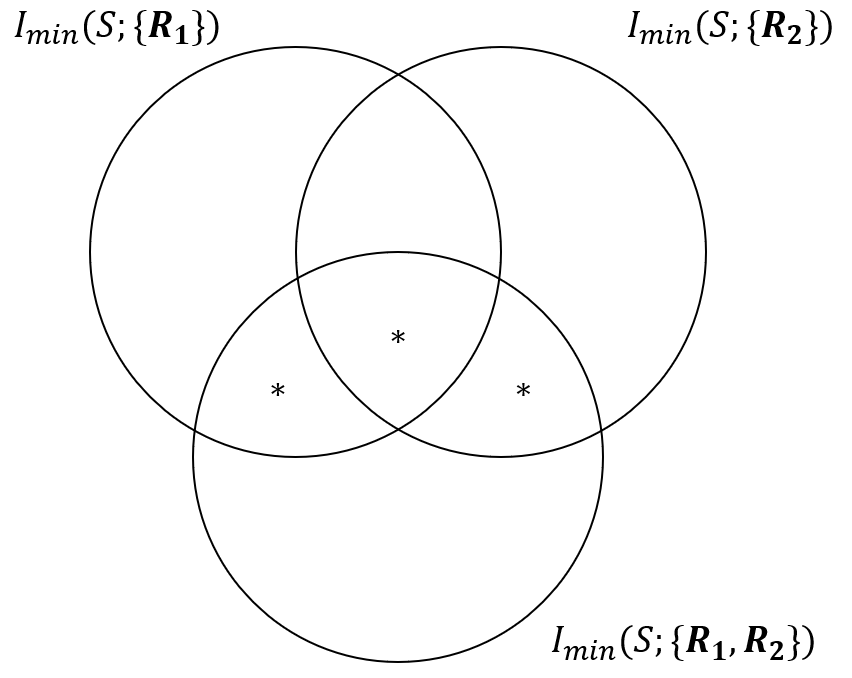
\includegraphics[height=4.5cm]{img/elim1.png}
%\caption{fig1}
\end{minipage}%
}%
\subfigure[After Elimination]{
\begin{minipage}[t]{0.5\linewidth}
\centering
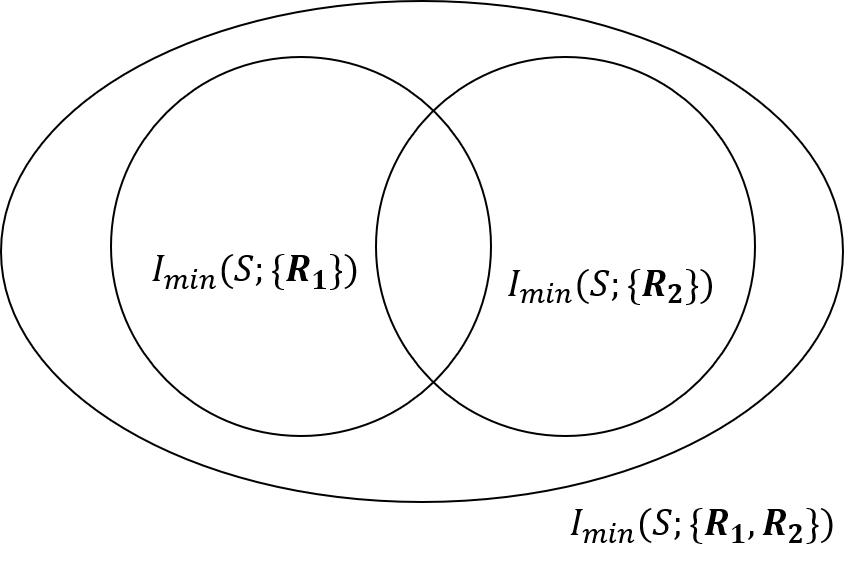
\includegraphics[height=4.5cm]{img/elim2.png}
%\caption{fig2}
\end{minipage}%
}%
\centering
\caption{Field Elimination for 2 Source Variables}
\label{fig:elim3}
\end{figure}

As the number of variables increases, the complexity of the combination also grows exponentially. It becomes nontrivial to identify all the subset relations, especially when higher-order fields are generated. Here is a formulated rule to follow.

\begin{theorem}[Field Elimination] For any two basic sets $\tilde{A}_{i\ldots j} , \tilde{A}_{i' \ldots j'} \in \Gamma$, if $\tilde{A}_{i\ldots j} \subseteq \tilde{A}_{i' \ldots j'}$, then the measure of any set intersection with $\tilde{A}_{i\ldots j} \cap \tilde{A}_{i' \ldots j'}^{C}$ is zero.
\begin{proof}
 The proof that $\mu^{*}\left( \left\{ \tilde{A}_{i\ldots j} \right\} \cap \left\{\tilde{A}_{i'\ldots j'} \right\}^{C} \right) = 0$ follows a similar pattern as Equation \ref{eqn:fieldelim}. For any set $\eta$ that intersects with $ \left\{ \tilde{A}_{i\ldots j} \right\} \cap \left\{\tilde{A}_{i'\ldots j'} \right\}^{C}$, by the non-negativity of partial information measure, we have
  \begin{equation}
     0 \le \mu^{*}\left(\eta  \cap \left\{ \tilde{A}_{i\ldots j} \right\} \cap \left\{\tilde{A}_{i'\ldots j'} \right\}^{C} \right) \le \mu^{*}\left( \left\{ \tilde{A}_{i\ldots j} \right\} \cap \left\{\tilde{A}_{i'\ldots j'} \right\}^{C} \right) = 0
\end{equation}
\end{proof}
\end{theorem}

The above theorem also implies a strategy to plot a pretty partial information diagram. Starting with singleton basic sets, every time we draw a new basic set, check the subset relation with the existing sets and eliminate the intersecting fields out. A construction of partial information diagram for four random variables is shown in Figure \ref{fig:elim4}. With such strategy, we can make clear how the partial information diagram in Figure \ref{fig:pidiagram} is step-by-step formulated with a set theoretic view.


\begin{figure}
\centering
\subfigure[$\tilde{A}_3$ produces no extra redundant fields]{
\begin{minipage}[t]{0.3\linewidth}
\centering
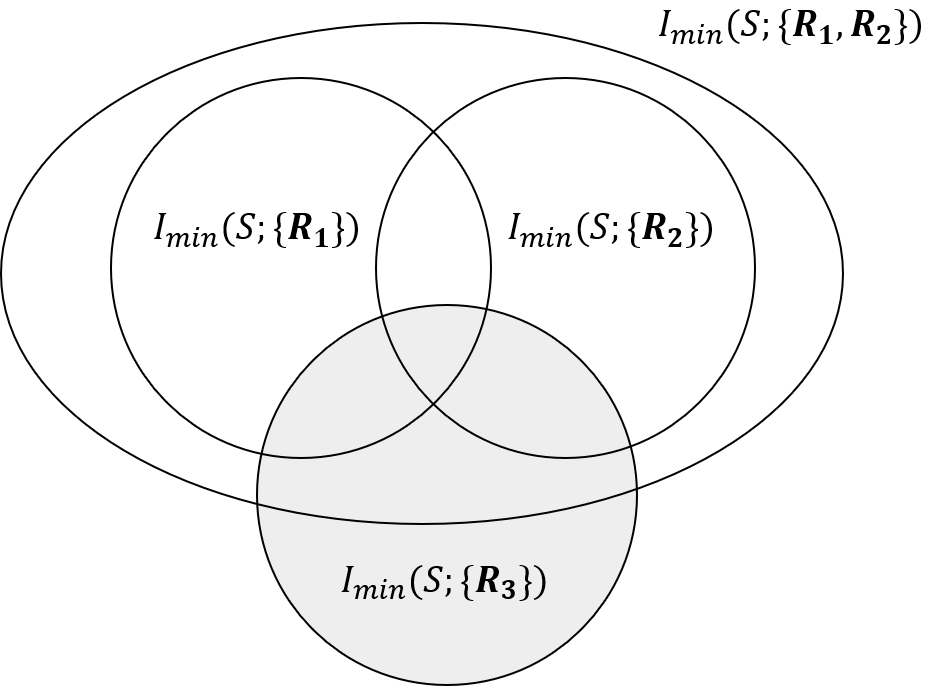
\includegraphics[height=3.5cm]{img/decompose1.png}
%\caption{fig1}
\end{minipage}%
}%
\quad
\subfigure[Adding Basic Set $\tilde{A}_{12}$ produces extra redundant fields as has been starred]{
\begin{minipage}[t]{0.3\linewidth}
\centering
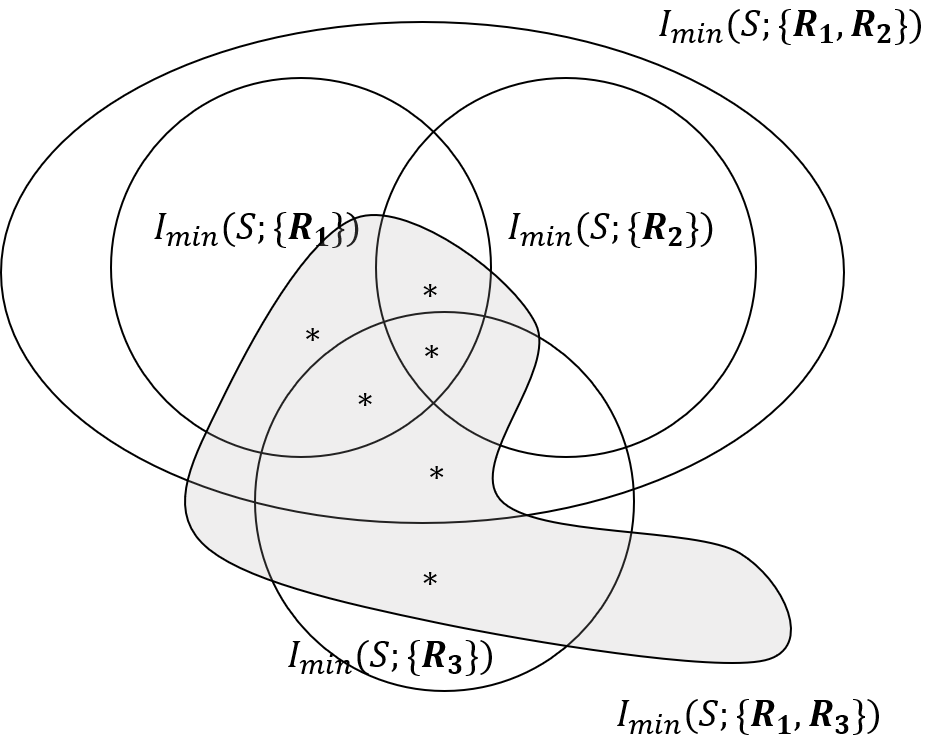
\includegraphics[height=3.5cm]{img/decompose2.png}
%\caption{fig2}
\end{minipage}%
}%
\quad
\subfigure[After Elimination]{
\begin{minipage}[t]{0.3\linewidth}
\centering
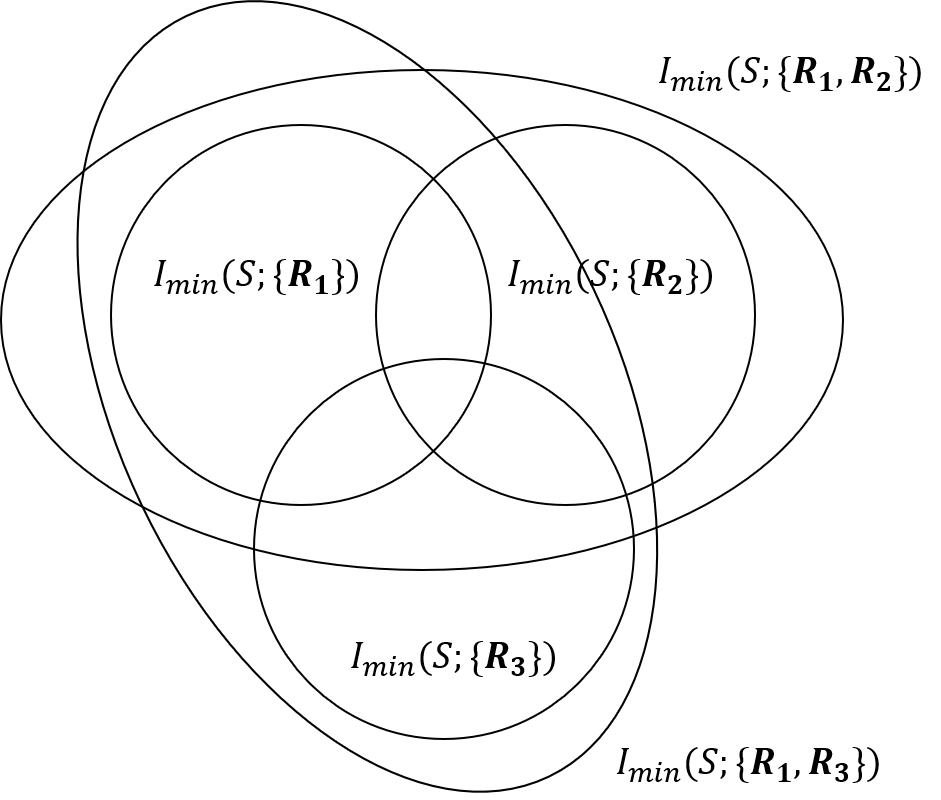
\includegraphics[height=3.5cm]{img/decompose3.png}
%\caption{fig2}
\end{minipage}%
}%
\centering
\caption{Field Elimination Strategy for 3 Source Variables}
\label{fig:elim4}
\end{figure}


\paragraph{Alternative Field Expressions} Note that the partial information $\Pi_{\mathbf{R}}$ is actually a derived concept. In common cases, we are more interested in the redundancy measure, which has more practical implications. We try to derive the relation between arbitrary field and linear combinations of redundancy measure from a pure set-theoretic view.

% Similar to Shannon information measure, we can define the \textit{universal set}
% \begin{equation}
%     \Omega = \bigcup_{i\in\mathcal{N}_n} \tilde{A}_i
% \end{equation} where the index set $\mathcal{N}_n$ is defined as

% \begin{equation}
%     \mathcal{N}_n = \mathcal{P}_1\left(\left\{ 1,2,\ldots,n\right\}\right)
% \end{equation}


Note that the measure of \textit{atoms} in $\mathcal{F}_n$ are a perfect matching to the partial information $\Pi_{\mathbf{R}}$. The reason is that by Definition \ref{def:partial}, $\Pi_\mathbf{R}\left(S;\alpha\right)$ only provides the unique information from $\alpha$. There is no possibility that the sets corresponding to a single partial information can be deposed to smaller sets by intersection, which coincides with the property of set atoms.

With the observation above, we can narrow our scope into atoms, since the measure of arbitrary set can be written into a combination of atoms. Because all atoms can be represented as sets of 

\begin{equation}
    \cap _{i\in\mathcal{N}_n} \tilde{Y}_i (\tilde{Y}_i = \tilde{A}_i \text{ or } \tilde{A}_i^c), \text{ where the index set } \mathcal{N}_n = \mathcal{P}_1\left(\left\{ 1,2,\ldots,n\right\}\right)
\end{equation}

we only need to study two operations, namely complement and intersection,  on basic sets $Y_{i \in \mathcal{N}_n}$. The mapping of such operations to redundancy measures can be listed as follows.

\begin{align}
    & \mu^{*}\left( \tilde{A}_{N_1} \cap \ldots \cap \tilde{A}_{N_k} \cap \tilde{A}_{M_1}^{C} \cap \ldots\cap \tilde{A}_{M_j}^{C} \right) \\
    &= \mu^{*}\left(\tilde{A}_{N_1} \cap \ldots \cap \tilde{A}_{N_k} \right) - \sum_{i=1}^{k} \mu^{*} \left( \tilde{A}_{N_1} \cap \ldots \cap \tilde{A}_{N_k} \cap\tilde{A}_{M_1} \cap \ldots \cap \tilde{A}_{M_i} \right) \label{eqn:simplify} \\  
    & \text{where } \left\{ N_1, \ldots, N_k, M_1, \ldots, M_k \right\} = \mathcal{N}_n \label{eqn:idxsetatom}
\end{align}

The formula above is not hard to obtain from a pure set-theoretic perspective, now note that in Equation \ref{eqn:simplify}, all the sets being measured are intersections of basic sets. By applying Equation \ref{eqn:intersectofbasic}, we can write them out in the form of redundancy measure $I_{\min}$. By now, we have finished proving that any atom can be written as a $\pm 1$ combination of some redundancy measures.

Therefore, we can conclude that any field can be written as
a linear combination of redundancy measures. An application of such expression is to calculate partial information in a top-down way. In the next chapter we will apply such strategy to show how our method can eliminate the need to calculate lots of partial information in the traditional bottom-up strategy.

Note that if we change the equality into $\subseteq$ in Equation \ref{eqn:idxsetatom}, the formula will still hold, i.e. we can always write out the intersection of any basic sets or their complements in the form of Equation \ref{eqn:simplify}, which may help us reduce the complexity of computing redundancy a step further.

\subsection{Completeness}
In order to validate the effectiveness of the PI-measure correspondence, we will close our formulation section with a conclusion that the measure of any field can be completely obtained from the measures of basic sets.


\begin{theorem}
Let
\begin{equation}
    \mathcal{B} = \left\{ \tilde{X}_{G}: G \text{ is a nonempty subset of  }\mathcal{N}_n \right\}
\end{equation}
Then a measure $\mu^{*}$ on $\mathcal{F}_n$ is completely specified by $\left\{ \mu^{*}(B), B \in \mathcal{B} \right\}$, which can be any set of real numbers.

\begin{proof}
The number of elements in $\mathcal{B}$ is equal to the number of nonempty subsets of $\mathcal{N}_{n},$ which is $2^{2^{n}-1}-1 .$ Thus $|\mathcal{A}|=|\mathcal{B}|=2^{2^{n}-1}-1  .$ Let $k=2^{2^{n}-1}-1 $ Let $\mathbf{u}$ be a column $k$ -vector of $\mu(A), A \in \mathcal{A},$ and $\mathbf{h}$ be a column $k$ -vector of $\mu(B), B \in \mathcal{B} .$ since all the sets in $\mathcal{B}$ can expressed uniquely as the union of some nonempty atoms in $\mathcal{A},$ by the set-additivity of $\mu,$ for each $B \in \mathcal{B}, \mu(B)$ can be expressed uniquely as the sum of some components of u. Thus
\begin{equation}
\mathbf{h}=C_{n} \mathbf{u}
\label{eqn:completeness1}
\end{equation}
where $C_{n}$ is a unique $k \times k$ matrix. On the other hand, it has been shown that for each $A \in \mathcal{A}, \mu^{*}(A)$ can be expressed as a linear combination of $\mu(B), B \in \mathcal{B}$ by applications, if necessary, of Equation \ref{eqn:simplify}.

However, the existence of the said expression does not imply its uniqueness. Nevertheless, we can write
\begin{equation}
\mathbf{u}=D_{n} \mathbf{h}
\label{eqn:completeness2}
\end{equation}
for some $k \times k$ matrix $D_{n} .$ Upon substituting Equation \ref{eqn:completeness1} into Equation \ref{eqn:completeness2}, we obtain
\begin{equation}
\mathbf{u}=\left(D_{n} C_{n}\right) \mathbf{u}
\label{eqn:completeness3}
\end{equation}
which implies that $D_{n}$ is the inverse of $C_{n}$ as Equation \ref{eqn:completeness3} holds regardless of the choice of $\mu .$ since $C_{n}$ is unique, so is $D_{n} .$ Therefore, $\mu^{*}(A), A \in \mathcal{A}$ are uniquely determined once $\mu^{*}(B), B \in \mathcal{B}$ are specified. Hence, a measure $\mu^{*}$ on $\mathcal{F}_{n}$ is completely specified by $\{\mu(B), B \in \mathcal{B}\},$ which can be any set of real numbers. The theorem is proved.

\end{proof}

\end{theorem}

\section{Application}

% another way to calculate $\Pi_{\mathrm{R}}$
In Chapter 4, we introduce the measure of partial information, which successfully captures the unique information provided by every possible combination of sources. Then we know the total information provided by a source can be divided into several partial information contributions, because the mutual information becomes a sum of these partial information terms.\\

Here we introduce the application of our theories. We try to calculate the value of any $\Pi_{\mathrm{R}}$ in two ways. On one hand, we can use the original definition of $\Pi_{\mathrm{R}}$ to calculate, by applying Equation \ref{ee1}. On the other hand, we can calculate $\Pi_{\mathrm{R}}$ by converting it to the linear combination of $I_{\min}$ with our strategy proposed above. 

\paragraph{Three Variables}
First consider the simplest case of a system with three variables: S,${R_1}$ and ${R_2}$, we want to calculate the value of $\Pi_{\mathrm{R}}(S ; \{1\})$.

With the original definition, we can apply $\beta=\{\{1\}\{2\}\}$ to the following Equation \begin{equation}\Pi_{\mathbf{R}}(S ; \alpha)=I_{\min }(S ; \alpha)-\sum_{s} p(s) \max _{\beta \in \alpha^{-}} \min _{\mathbf{B} \in \beta} I(S=s ; \mathbf{B})
\label{ee1}
\end{equation}  to get
\begin{equation}\Pi_{\mathbf{R}}(S ;  \{1\})=I_{\min }(S ; \{1\})-I_{\min }(S ;\{1\}\{2\})\label{ee2}\end{equation}

Use our theorem, based on the observations in Figure \ref{fig:pidiagram}(a), we can express the field using Equation \ref{eqn:intersectofbasic}:
\begin{equation}
\begin{aligned}
    \mu^{*}\left( \left\{ \tilde{R}_1 \right\} \cap \left\{ \tilde{R}_2 \right\}^{C} \cap \left\{\tilde{R}_1, \tilde{R}_2 \right\} \right) &= \mu^{*}\left(\left\{\tilde{R}_1 \right\}\cap  \left\{  \tilde{R}_1, \tilde{R_2} \right \} \right)  -\mu^{*}\left( \left\{\tilde{R}_1\right\}\cap \left\{ \tilde{R}_2 \right\}\cap \left\{\tilde{R}_1, \tilde{R}_2 \right\}\right) \\
    &=I_{\min} \left( S; \left\{ 1 \right\} ,\left\{ 1, 2 \right\} \right)  - I_{\min} \left( S; \left\{1 \right\}, \left\{2 \right\},\left\{ 1, 2 \right\} \right) \\&=I_{\min} \left( S; \left\{ 1 \right\}  \right)  - I_{\min} \left( S; \left\{1 \right\}, \left\{2 \right\} \right)
\end{aligned}
\label{ss}
\end{equation}

where the last equality holds because $\left\{ \tilde{R}_1 \right\} \subseteq \left\{\tilde{R}_1, \tilde{R}_2 \right\}$.\\

We can show the equivalence of the two methods with a simple example. In Figure\ref{fig8}, the black tiles represent equally-probable outcomes and the white tiles are zero-probability outcomes. Using the formula below
\begin{equation}
\begin{aligned}
    I(S ; \mathbf{A}) &=\sum_{s} p(s) I(S=s ; \mathbf{A}) \\
    I(S=s ; \mathbf{A}) &=\sum_{\mathbf{a}} p(\mathbf{a} | s)\left[\log \frac{1}{p(s)}-\log \frac{1}{p(s | \mathbf{a})}\right] \\
    I_{\min }\left(S ;\left\{\mathbf{A}_{1}, \mathbf{A}_{2}, \ldots, \mathbf{A}_{k}\right\}\right)&=\sum_{s} p(s) \min _{\mathbf{A}_{i}} I\left(S=s ; \mathbf{A}_{i}\right)
\end{aligned}
\end{equation}

we can calculate that $I\left(S ; \{1\}\right)=I\left(S ; \{2\}\right)=-\frac{1}{3} \log \frac{1}{3}-\frac{2}{3} \log \frac{2}{3}$, and $I_{\min }(S ; \{1\},\{2\})=\log 3-\log 2$.\\
Finally, we have $\Pi_{\mathbf{R}}(S ; \{1\})=-\frac{1}{3} \log \frac{1}{3}-\frac{2}{3} \log \frac{2}{3}-\log 3+\log 2=\frac{1}{3}$.

\begin{figure}[ht]
 
\centering
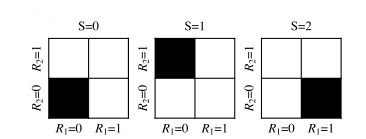
\includegraphics[height=4cm]{tex/example.jpg}
\caption{Probability distributions for $S\in\{0,1,2\}$ and$R_1,R_2\in\{0,1\}$.}
\label{fig8}
 
\end{figure}

\paragraph{Four Variables}
Now we consider a more complicated system with four variables, and we want to calculate the value of $\Pi_{\mathrm{R}}(S ; \{2\},\{13\})$.

On one hand, we can apply Equation \ref{ee1}  to solve the problem:
\begin{equation}\Pi_{\mathbf{R}}(S ;\{2\},\{13\})=I_{\min }(S ; \{2\},\{13\})-\sum_{s} p(s) \max _{\beta \in \alpha^{-}} \min _{\mathbf{B} \in \beta} I(S=s ; \mathbf{B})\label{43}\end{equation} 
where $\beta \in\{\{\{1\}\{2\}\},\{\{2\}\{3\}\}\} $ . Then we just need to expand the formula to get the result. 

On the other hand, based on the observations in Figure\ref{fig:pidiagram}(b), we can express the field using Equation \ref{eqn:intersectofbasic}:


\begin{equation}
    \begin{aligned}
    &\mu^{*}\left( \left\{ \tilde{R}_1 \right\}^{C} \cap \left\{ \tilde{R}_2 \right\}\cap \left\{ \tilde{R}_3 \right\}^{C} \cap \left\{\tilde{R}_{12} \right\}\cap \left\{\tilde{R}_{13} \right\}\cap \left\{\tilde{R}_{23} \right\}\cap \left\{\tilde{R}_{123} \right\} \right)  \\
   =&\mu^{*}\left(\left\{\tilde{R}_2 \right\}\cap  \left\{  \tilde{R}_{12} \right \}\cap  \left\{  \tilde{R}_{13} \right \} \cap  \left\{  \tilde{R}_{23} \right \}\cap \left\{\tilde{R}_{123} \right\}\right)  -\mu^{*}\left(\left\{\tilde{R}_1 \right\}\cap \left\{ \tilde{R}_2 \right\}\cap  \left\{  \tilde{R}_{12} \right \}\cap  \left\{  \tilde{R}_{13} \right \}\cap  \left\{  \tilde{R}_{23} \right \}\cap \left\{\tilde{R}_{123} \right\}\right)\\
    &-\mu^{*}\left(\left\{\tilde{R}_2 \right\}\cap \left\{ \tilde{R}_3 \right\}\cap  \left\{  \tilde{R}_{12} \right \}\cap  \left\{  \tilde{R}_{13} \right \} \cap  \left\{  \tilde{R}_{23} \right \}\cap \left\{\tilde{R}_{123} \right\}\right) \\
    &+\mu^{*}\left( \left\{ \tilde{R}_1 \right\} \cap \left\{ \tilde{R}_2 \right\}\cap \left\{ \tilde{R}_3 \right\} \cap \left\{\tilde{R}_{12} \right\}\cap \left\{\tilde{R}_{13} \right\}\cap \left\{\tilde{R}_{23} \right\}\cap \left\{\tilde{R}_{123} \right\} \right)\\
    =&I_{\min} \left( S; \left\{ 2 \right\} ,\left\{ 1, 2 \right\} ,\left\{ 1, 3 \right\},\left\{ 2, 3 \right\},\left\{ 1, 2, 3 \right\}\right)  - I_{\min} \left( S; \left\{ 1 \right\} ,\left\{ 2 \right\} ,\left\{ 1, 2 \right\} ,\left\{ 1, 3 \right\},\left\{ 2, 3 \right\},\left\{ 1, 2, 3 \right\}\right) \\
    &- I_{\min} \left( S; \left\{ 2 \right\} ,\left\{ 3 \right\} ,\left\{ 1, 2 \right\} ,\left\{ 1, 3 \right\},\left\{ 2, 3 \right\},\left\{ 1, 2, 3 \right\}\right) +I_{\min} \left( S; \left\{ 1 \right\} ,\left\{ 2 \right\} ,\left\{ 3 \right\} ,\left\{ 1, 2 \right\} ,\left\{ 1, 3 \right\},\left\{ 2, 3 \right\},\left\{ 1, 2, 3 \right\}\right)\\
    =&I_{\min} \left( S; \left\{ 2 \right\} ,\left\{ 1, 3 \right\}\right)  - I_{\min} \left( S; \left\{ 1 \right\} ,\left\{ 2 \right\} \right) - I_{\min} \left( S; \left\{ 2 \right\} ,\left\{ 3 \right\} \right) +I_{\min} \left( S; \left\{ 1 \right\} ,\left\{ 2 \right\} ,\left\{ 3 \right\} \right)
    \end{aligned}
\end{equation}


By some set operations, it can be translated into the linear combination of $I_{\min}$. The last equality holds because the former can be greatly simplified. For example, $\left\{ \tilde{R}_2 \right\} \subseteq \left\{\tilde{R}_1, \tilde{R}_2 \right\},\left\{\tilde{R}_2, \tilde{R}_3 \right\}\cdots$Now we just need to calculate the value of each $I_{min}$.\\

% What's more, we can also get the result applying Equation \ref{def:partial}, by which we can express $\Pi_{\mathbf{R}}$ using the linear combination of $I_{\min}$.\\

% We can list all $I_{\min}$ of the  sets which have the partial order relation with $\{\{2\},\{13\}\}$:

% \begin{equation}I_{\min }(S;\left\{2\},\{13\}\right)=\Pi_{\mathbf{R}}(S ;\{2\},\{3\})+\Pi_{\mathbf{R}}(S ;\{1\},\{2\})+\Pi_{\mathbf{R}}(S ;\{2\},\{13\})+I_{\min }(S;\left\{1\},\{2\},\{3\}\right)\label{44}\end{equation}

% \begin{equation}I_{\min }(S;\left\{2\},\{3\}\right)=\Pi_{\mathbf{R}}(S ;\{2\},\{3\})+I_{\min }(S;\left\{1\},\{2\},\{3\}\right)\label{45}\end{equation}

% \begin{equation}I_{\min }(S;\left\{1\},\{2\}\right)=\Pi_{\mathbf{R}}(S ;\{1\},\{2\})+I_{\min }(S;\left\{1\},\{2\},\{3\}\right)\label{46}\end{equation}

% Combine Equation \ref{44},\ref{45},\ref{46}, then we have the save result as before.\\

Now we use another simple example to illustrate the equivalence between the two expressions. Based on the probability distribution in Figure \ref{fig8}, we introduce another variable $R_3$. Consider the equally-probable cases of S as follows:
\[
\begin{array}{c}
S=0 \iff {R}_1=0,{R}_2=0,{R}_3=0\\
S=1 \iff {R}_1=0,{R}_2=1,{R}_3=1\\
S=2 \iff {R}_1=1,{R}_2=0,{R}_3=0\\
\end{array}
\]

On one hand, by applying Equation \ref{43}, we have
\begin{equation}I_{\min }(S ; \{2\},\{13\})=\log3 -\frac{2}{3} \log 2\end{equation}
\begin{equation}\sum_{s} p(s) \max _{\beta \in \alpha^{-}} \min _{\mathbf{B} \in \beta} I(S=s ; \mathbf{B})=\log3 -\frac{2}{3} \log 2\end{equation}
So $\Pi_{\mathrm{R}}(S ; \{2\},\{13\})$=0.\\

On the other hand, by calculating by the linear combination of $I_{\min}$, we can also have the same outcome. In other words,
\begin{equation}I_{\min} \left( S; \left\{ 1 \right\} ,\left\{ 2 \right\} \right) - I_{\min} \left( S; \left\{ 2 \right\} ,\left\{ 3 \right\} \right) +I_{\min} \left( S; \left\{ 1 \right\} ,\left\{ 2 \right\} ,\left\{ 3 \right\}\right)=\sum_{s} p(s) \max _{\beta \in \alpha^{-}} \min _{\mathbf{B} \in \beta} I(S=s ; \mathbf{B})\end{equation}




\section{Discussion}

In this project, we first revisited I-Measure, a correspondence between Shannon's information and set theory. Then we introduced redundancy measure, together with its decomposed form, partial information, a non-negative measure in describing the redundancy a multivariate collection of sources provide for a particular random variable.

Inspired by I-Measure, we formally defined ``PI-Measure'' in the scope of set theory to formally describe how partial information diagrams are formed. We formulate the correspondence rules between PI-Measure and gave out its correspondence with partial information and redundancy measure. Then we made some simplifications to eliminate redundant fields. We've also found a strategy to find alternative expressions on partial information from a pure set-theoretic perspective. Finally, we calculated the partial information for some simple examples to compare our proposed strategy with the existing one.

We hope that our formulation can help clarify and substantiate how partial information diagrams are generated and can be used.





\printbibliography


\end{document}
